% !TeX root = ../../thesis.tex

\section{Neither Secure Boot nor Bitlocker}
% first aim harddrive access
The first attack is performed without enabling any security mechanisms (e.g. Secure Boot, BitLocker). Our first step is to gain unrestricted access to the hard drive from the UEFI environment.
% windows uses NTFS
Since Windows uses NTFS formatting for their hard drive volumes we need to use an NTFS driver, UEFI is not required to support NTFS and as such edk2 does not come with an NTFS driver.

% search for UEFI NTFS driver with write access
% open source fork of ntfs-3g for UEFI
Luckily open source NTFS drivers are readily available such as ntfs-3g from tuxera \cite{ntfs-3g} which allow for read and write access, on top of that there already exists a port to UEFI created by pbatard \cite{ntfs-3g-uefi}.

% compile
% spits out .efi file
We can compile this driver with edk2 following the listed steps and receive a .efi file.

% try in EFI shell
% what is the EFI shell
\TODO{better summary of UEFI shell}
Part of the UEFI specifications is a shell specification which is a feature rich UEFI shell application to interact with the UEFI environment.
% https://docstore.mik.ua/manuals/hp-ux/en/5991-1247B/ch04s13.html
\TODO{better listing of capabilities}
It offers commands for
boot,
configuration,
device, driver, handle
filesystem
network
memory
scripting.
For now driver loading and filesystem navigation are of relevance.

% how to use uefi shell
\TODO{look up official guideline to booting into console}
% we are trying in qemu where the shell is available in boot options
% real hardware might require the uefi shell application .efi from the user via usb stick
The UEFI shell can be part of the boot options or requires the user to supply the executable via a removable medium such as a USB stick.

% explain shell screen
Upon invocation, the shell application performs an initialization during which it \TODO{whats important for us here} and produces output that is equivalent to the output of the execution of the commands ver and map -terse \cite[3.3 Initialization]{uefi-shell}. ver displays the version of the UEFI specification the firmware conforms to \cite[5.3 Shell Commands]{uefi-shell}.

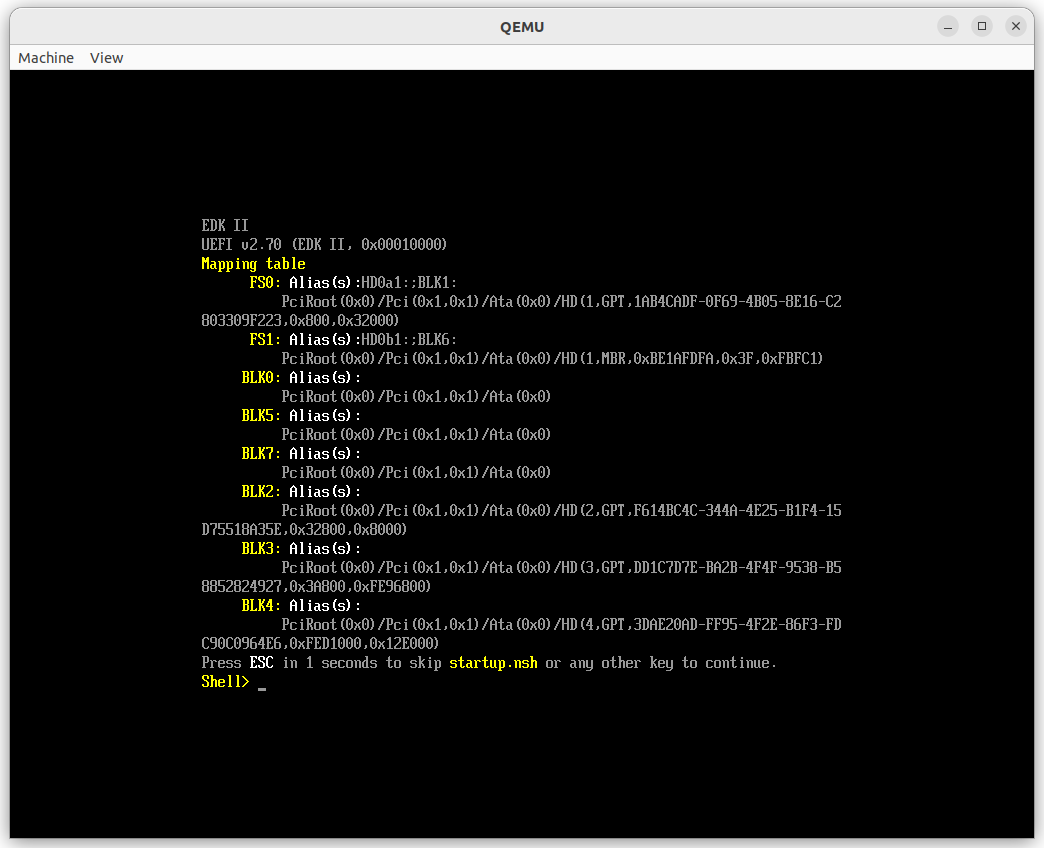
\includegraphics[width=\textwidth]{unsecure/qemu/01_uefi_shell.png}


% showing mapping, also available with map command
% consistent device mapping, comparable to partition names in windows
The map command is very interesting for file access with the shell, it displays a mapping table between user defined alias names and device handles. The aliases can be used instead of a device path when submitting commands via the command line interface. The UEFI shell also produces default mappings, notably for file systems \cite[3.7.2. Mappings]{uefi-shell}. These mappings are designed to be consistent across reboots as long as the hardware configuration stays the same, they are comparable to Windows partition letters. \cite[Appendix A]{uefi-shell}

% blk and fs
\TODO{find in spec what precise mapping mechanism}
When we inspect the mapping table we can see FSx and BLKx aliases, FSx maps to file systems and BLKx to block devices. THis identification is performed via instances of the Simple File System Protocol and \TODO{double check} Block I/O Protocol which present the interfaces to access the devices they are installed to.
% explain Simple File System Protocol
The Simple File System Protocol \cite[13.4 Simple File System Protocol]{uefi-spec} provides, together with the File Protocol, file-type access to the device it is installed on. The two protocols are independent of the underlying file system the media is formatted with.
\TODO{UEFI supported fule systems}
By default UEFI supports

\TODO{explain file system indepent abstraction better}
Drivers providing these protocols use the Block I/O Protocol to access the underlying media.


% load NtfsDxe.efi
Our NTFS UEFI Driver is one such abstraction and needs to be loaded now, this is done first entering alias, for the file system containing the NtfsDxe.efi, followed by a colon.
\TODO{alias for fs eingeben was macht das}
This effectively switches the console's working directory to be the root of the entered file system, now we caninvoke load with the path to the executable. The output indicates whether loading the driver was successful.
% drivers
% We can now list
\TODO{maybe better command here}
With the command drivers, we can list all currently loaded drivers and some basic information about them, such as number of devices managed. We can see that the NTFS driver already manages devices.

% map -r "reset all the default mappings in a system this option is useful if the system configuration has changed since the last boot"
% new mapping and fs ontop of old blk
\TODO{reword maybe move the block device stuff up}
We can now reset all default mappings with the map -r command to receive an updated list including the file system now provided by the NTFS driver. The mapping also shows us that the file system now sits on top of a device which previously was only listed as a block device indicating that the NTFS driver uses this block-wise access to offer the Simple File System Protocol.

As done before we now type the alias of the new file system followed with a colon to switch to NTFS formatted file system. With ls we can list the current directory's content and confirm by the presence of the Windows folder that we are on the volume containing the Windows installation.


% navigate to Windows folder
% means read works
% try creating folder to test write
We now navigate into the Windows folder to test whether we have unrestricted read and write access, since is not the case if done by an unprivileged user when performed from within Windows. Accessing folders and viewing their contents is possible but creation of a new folder fails.

% debug why it failed
% find out its from windows having hibernation enabled by default
% change source code to not fallback to read only when encountering hibernation file
Upon debugging the NTFS driver it appears to be that the drivers falls back to read only when it encounters a file that indicates that the Windows system is in hibernation mode. Windows seems to have hibernation enabled by default and as such our rootkit should not rely on it being disabled, we can change the code of the NTFS driver to not fallback when encountering this file.

We now know that provided we get to load the NTFS driver we can access a Windows installation and subsequently the entire data of unencrypted hard drives. Since our rootkit will not use the UEFI shell we need to have the NTFS driver load as part of the boot process.
% try to package in firmware image instead of loading from external medium
We can put the NTFS driver into the DXE Volume where the DXE Dispatcher of the DXE Core will automatically try to load it.

retrieve the image
for qemu we can build it ourselves
for hardware use spi clamp to  dump image

we can open image with UEFITool
an editor for firmware images conforming to the UEFI PI spec \cite{uefitool}

in UEFITool search for DXE Volume
remove previous NTFS driver if present, for full control, might be read only etc
in UEFITool search for string
since files are part of file sections we cant drop in the .efi
compile dxe driver within ovmf
generate unused volume to receive .ffs file with version, depex, user interface and pe section
add in NTFS driver .ffs file
qemu just use path to modified image
on hardware use write access with clamp

now upon opening uefi shell
we instantly see the filesystem

try to use ntfs-driver in code
this is our first rootkit iteration
payload will also be DXE driver
access to all drivers etc
package payload in firmware image
load after NTFS driver
install tag protocol on NTFS driver and put into depex of rootkit
steps
read payload into RAM
search for windows installation
write payload

pack executable binary as uefi module
edk2 produces freeform image with one raw section

iterate over FirmwareVolume2 protocol instances
boottime services offer a function LocateHandleBuffer which returns all handles having a given protocol attached to them
iterate over all handles and open the protocol
call ReadSection with payload guid, to read raw section
check size match was necessary on hardware
when compiling payload a post build script generates a header for the rootkit dxe containing the size on disk for the payload

iterate over all FirmwareVolume2 Protocols
read raw section of payload file GUID into memory

iterate over all SimpleFileSystem Protocols
open volume
open file to write to
since we write into windows folder this also checks if the volume has a windows installation

achieved so far unrestricted file access
but no automatic execution nor elevated privileges

% ref to background UAC signed
dll proxying
dll hijacking
registry editing

Task Scheduler
defined in xml
cached in registry
edit with start cmd.exe and trigger manually
whoami

chntpw and reged
\cite{chntpw}
port to uefi
edit Task in machine under Control
maybe look if just adding a key would have also worked
export target registry key
modify so that registry key can differ and found via matching values
import and override registry key on target machine
payload whoami
localsystem

